\documentclass[a4paper,10pt]{article}
\usepackage[utf8]{inputenc}
\usepackage{lipsum}
\usepackage{mathtools}
\usepackage{tikz}
\usepackage{pgfplots}
\usetikzlibrary{arrows,backgrounds,shapes,matrix,positioning,fit}
\usetikzlibrary{decorations.markings}
\usepackage{caption}
\usepackage{subcaption}
% For maths
\usepackage{amsmath}
% Set Margin
\usepackage[margin=1in]{geometry}
% For Figures
\usepackage{graphicx}
% For including source codes
\usepackage{listings}
\usepackage{color}
\definecolor{mygreen}{rgb}{0,0.6,0}
\definecolor{mygray}{rgb}{0.5,0.5,0.5}
\definecolor{mymauve}{rgb}{0.58,0,0.82}
\lstset{ %
  backgroundcolor=\color{white},   % choose the background color; you must add \usepackage{color} or \usepackage{xcolor}
  basicstyle=\footnotesize,        % the size of the fonts that are used for the code
  breakatwhitespace=false,         % sets if automatic breaks should only happen at whitespace
  breaklines=true,                 % sets automatic line breaking
  captionpos=b,                    % sets the caption-position to bottom
  commentstyle=\color{mygreen},    % comment style
  deletekeywords={...},            % if you want to delete keywords from the given language
  escapeinside={\%*}{*)},          % if you want to add LaTeX within your code
  extendedchars=true,              % lets you use non-ASCII characters; for 8-bits encodings only, does not work with UTF-8
  frame=single,                    % adds a frame around the code
  keepspaces=true,                 % keeps spaces in text, useful for keeping indentation of code (possibly needs columns=flexible)
  keywordstyle=\color{blue},       % keyword style
  language=Octave,                 % the language of the code
  morekeywords={*,...},            % if you want to add more keywords to the set
  numbers=left,                    % where to put the line-numbers; possible values are (none, left, right)
  numbersep=5pt,                   % how far the line-numbers are from the code
  numberstyle=\tiny\color{mygray}, % the style that is used for the line-numbers
  rulecolor=\color{black},         % if not set, the frame-color may be changed on line-breaks within not-black text (e.g. comments (green here))
  showspaces=false,                % show spaces everywhere adding particular underscores; it overrides 'showstringspaces'
  showstringspaces=false,          % underline spaces within strings only
  showtabs=false,                  % show tabs within strings adding particular underscores
  stepnumber=2,                    % the step between two line-numbers. If it's 1, each line will be numbered
  stringstyle=\color{mymauve},     % string literal style
  tabsize=2,                       % sets default tabsize to 2 spaces
  title=\lstname                   % show the filename of files included with \lstinputlisting; also try caption instead of title
}
\usepackage{caption}
\usepackage{url}
% for appendix
\usepackage[toc,page]{appendix}
\begin{document}

\pgfplotsset{compat=1.3}

%\tableofcontents

%\chapter{GNU Radio}

\section{GNU Radio}
GNU Radio\cite{bib:gnuradio} is a free \& open-source software development toolkit
that provides signal processing blocks to implement software radios.
It can be used with readily-available low-cost external RF hardware
to create software-defined radios, or without hardware in a simulation-like environment.
It is widely used in hobbyist, academic and commercial environments 
to support both wireless communications research and real-world radio systems.

A software radio is a radio system which performs the required signal processing 
in software instead of using dedicated integrated circuits in hardware.
The benefit is that since software can be easily replaced in the radio system,
the same hardware can be used to create many kinds of radios for many different transmission standards;
thus, one software radio can used for a variety of applications.

GNU Radio performs all the signal processing.
You can use it to write applications to receive data out of digital streams 
or to push data into digital streams, which is then transmitted using hardware.
GNU Radio has filters, channel codes, synchronization elements, equalizers,
demodulators, vocoders, decoders, and many other elements 
(in the GNU Radio jargon, we call these elements blocks) which are typically found in radio systems.
More importantly, it includes a method of connecting these blocks 
and then manages how data is passed from one block to another.
Extending GNU Radio is also quite easy; if you find a specific block that is missing, you can quickly create and add it.

Since GNU Radio is software, it can only handle digital data.
Usually, complex baseband samples are the input data type for receivers and the output data type for transmitters.
Analog hardware is then used to shift the signal to the desired center frequency.
That requirement aside, any data type can be passed from one block to another 
- be it bits, bytes, vectors, bursts or more complex data types.

GNU Radio applications are primarily written using the Python programming language, 
while the supplied, performance-critical signal processing path is implemented in C++
using processor floating point extensions, where available.
GNU Radio Companion(GRC) is a Simulink-like graphical tool to design signal processing flow graphs.

GNU Radio supports several radio front-ends, either natively or through additional out-of-tree modules.
We will be using Ettus Research USRP platform and RTL-SDR TV tuners.

\subsection{First flow-graph}
Flow graphs are graphs (as in graph theory) through which data flows.
Many GNU Radio applications contain nothing other than a flow graph.
The nodes of such a graph are called blocks, and the data flows along the edges.

Any actual signal processing is done in the blocks.
Ideally, every block does exactly one job - this way GNU Radio stays modular and flexible.
Blocks are usually written in C++ (might also be Python); writing new blocks is not very difficult.

In order to illuminate this diffuse topic a little, let's start with an example.
Our aim is to generate a sinusoid and play it on audio output.
Open GNU Radio companion by executing gnuradio-companion on a terminal. 
The completed flow-graph is shown in Figure \ref{fig:audio-play1}.
\begin{figure}
\centering
 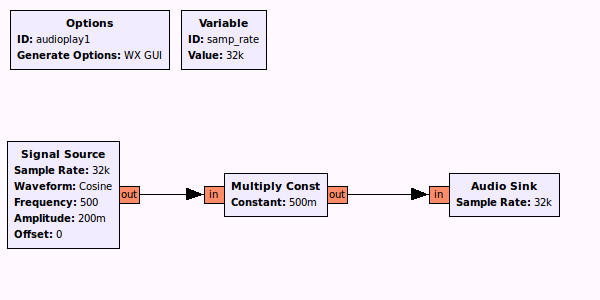
\includegraphics[scale=0.40]{figures/audio-play1.png}
 \caption{Playing 500Hz sinusoid on audio output.
 Take signal source and audio sink block from the list of blocks.
 Set the data type of signal source to float.
 Set the frequency to 500Hz and sampling rate to 32k.
 Set the sampling rate in the audio sink block to 32k.
 Connect these blocks and execute the flow-graph.\label{fig:audio-play1}}
\end{figure}

The blocks are connected at ports. 
The first block has no input port, it produces samples. 
Such a block, with only output ports, is called a source. 
In an analog fashion, the final block, with no outputs, is called a sink.

So what's happening here?
The signal source produces samples of 500Hz cosine sampled at 32kHz per second.
The first 64 samples (which corresponds to a complete cycle of cosine in this case)
is plotted in Figure \ref{fig:signal-source-out}.
These samples are consumed by the multiply constant block,
which multiplies each of the input with 0.5.
Finally, the samples are passed to the audio output block which plays the incoming samples using computers audio card.
\begin{figure}
 \centering
 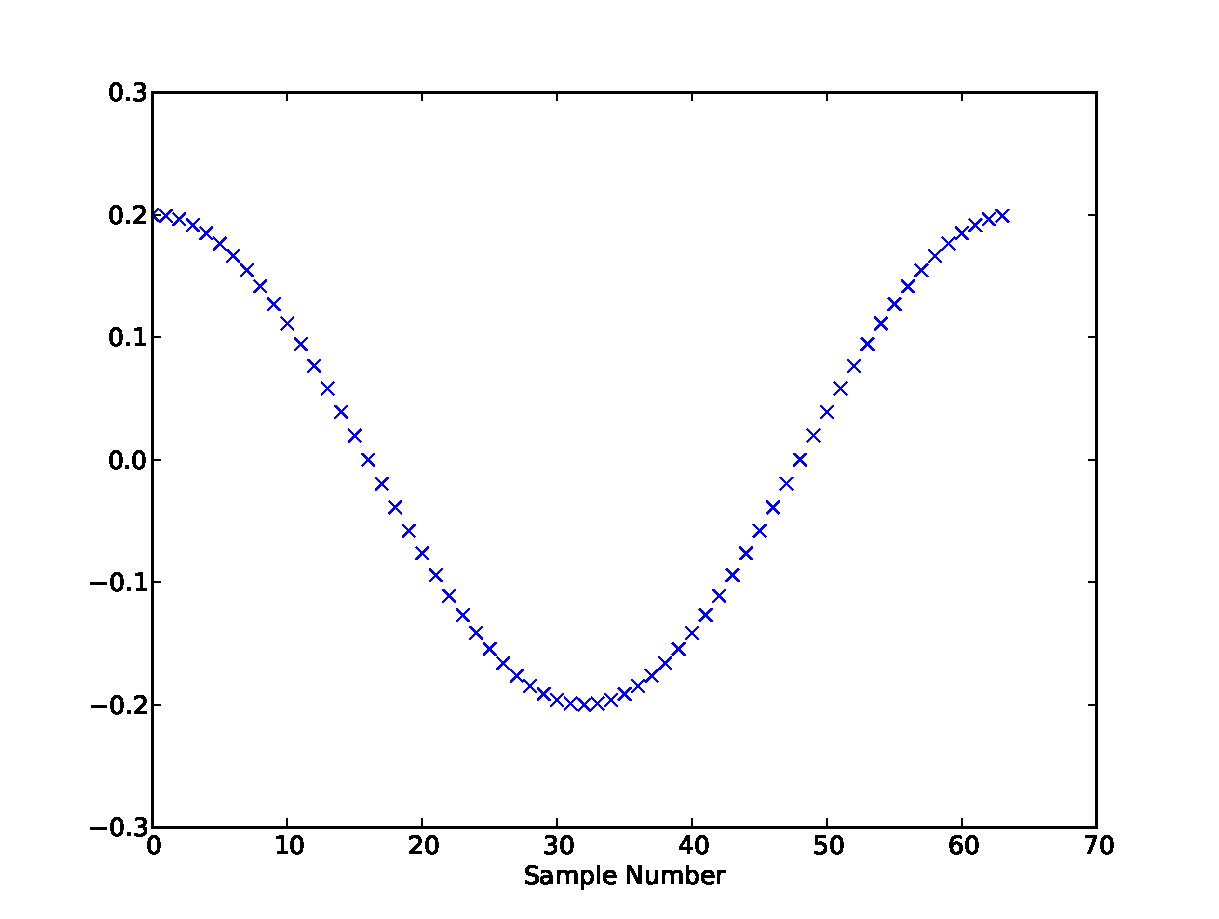
\includegraphics[scale=0.4]{figures/signal-source-out}
 \caption{The first 64 samples of output from the signal source. \label{fig:signal-source-out}}
\end{figure}

In general, we call whatever a block outputs an item. 
In Figure \ref{fig:audio-play1}, one item was a float value representing one sample produced by the signal source. 
However, an item can be anything that can be represented digitally. 
The most common types of samples are real samples (as before), complex samples (the most common type in software defined radio), integer types, and vectors of these scalar types.

In Figure \ref{fig:audio-play1}, apart from playing the samples on audio card, everything else is done in software.
Since the audio card can only take specific sampling rates(32kHz, 44.1kHz, etc)
the rate at which the samples are processed through this flow graph will be equal to the sampling rate of the audio card.
As mentioned before GNU Radio applications are written in python programming language. When we run any flow-graph
in GNU Radio companion, it is a python program that runs behind the scene. The python program corresponding to 
the flow-graph in Figure \ref{fig:audio-play1} is given in Listing \ref{lst:audio-play1}.
This program is auto-generated when we run a GNU Radio companion(GRC) flow graph.

Let us consider another example of computing the FFT of a signal source.
The flow graph is given in Figure \ref{fig:compute-fft}.
In this example, the second block (stream to vector) produces one item(which is a vector of 1024 complex number) for every 1024 input items.
So, the rate at which it produces items is 1024 times smaller then the rate at which it consumes items 
(the fact that it actually produces bytes at the same rate it consumes them is irrelevant here).
Such a block is called a decimator, well, because it decimates the item rate. 
A block which outputs more items than it receives is called an interpolator. 
If it produces and consumes at the same rate, it's a sync block.
\begin{figure}
 \centering
 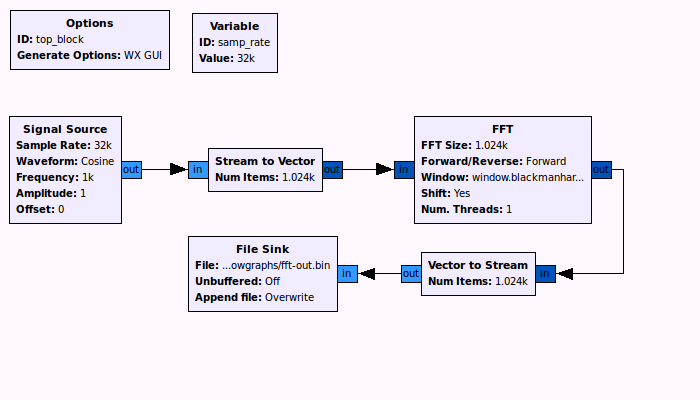
\includegraphics[scale=0.4]{figures/fft.png}
 \caption{Computing FFT \label{fig:compute-fft}}
\end{figure}

Let us ask the question what is the base sampling rate in Figure \ref{fig:compute-fft}?
Or how many complex numbers produced by the signal source, will be processed through this flow graph in a second?
Well, we can't really answer this question.
In this flow graph all that we are do, is to generate some numbers, do some math on the generated numbers, and save the output to a file.
As long as there is no hardware clock present which fixes the rate, 
sampling rate is meaningless--only relative rates (i.e. input to output rates are important. 
The computer may handle the samples as fast as it wants.
Note that this can cause the computer to lock up by allocating 100\% of CPU cycles to your signal processing.

In order to avoid the computer getting busy doing all the math, it is recommended to use a throttle block
when we run GNU Radio without any other hardware. The throttle block is tied to computer's hardware clock,
and it throttles the number of items passing through it.

Also when we have hardware involving different sampling rates, we might have to use some up-sampling/down-sampling
so that we meet the sampling rate requirement of all the hardwares.

\section{IQ Modulation\cite{bib:madhov}}
In RF communication we transmit our information in a small passband around a high frequency carrier.
All the information carried in a real-valued passband signal is contained in a corresponding complex-valued baseband signal. 
This baseband signal is called the complex baseband representation, or complex envelope, of the passband signal.
Any passband signal $s_{\text{p}}(t)$ can be written as
\begin{equation}
 s_{\text{p}}(t) = \sqrt{2}s_{\text{i}}(t)\operatorname{cos}(2\pi f_ct) - \sqrt{2}s_{\text{q}}(t)\operatorname{sin}(2\pi f_ct)
\end{equation}
where,
\begin{equation}
 s(t) = s_{\text{i}}(t) + \text{j}s_{\text{q}}(t)
\end{equation}
is called the complex envelope of $s_{\text{p}}(t)$. In GNU Radio we work with this complex envelope.
There are many hardwares available which can be interfaced with GNU Radio to transmit the output from a flow-graph
around any carrier that we may choose. Figure \ref{fig:complex-passband-spectrums} compares the spectrum of 
complex envelope and passband signals. Figure \ref{fig:upconversion} shows the process of IQ modulation.
Figure \ref{fig:downconversion} shows the process of IQ demodulation.

  \begin{figure}
    \centering
    \begin{subfigure}[t]{0.4\textwidth}
      \begin{tikzpicture}[scale=0.8,transform shape]
        \begin{axis}[
                     title=$\Re(S(f))$,
                     xmax=7,
                     xmin=-7,
                     ymax=1.5,
                     ymin=-1.1,
                     %axis lines = middle,
                     axis x line = middle,
                     axis y line = middle,
                     ytick=\empty,
                     xtick = {7},
                     xticklabels = {$f$},
                     %x tick label style={font=\tiny},
                     x post scale = 3.0
                    ]
          \addplot[color=blue,very thick] coordinates {(1,0) (-1,1.414) (-1,0)};
        \end{axis}
      \end{tikzpicture}
  \end{subfigure}
  \begin{subfigure}[t]{0.4\textwidth}
      \begin{tikzpicture}[scale=0.8,transform shape]
        \begin{axis}[
                     title=$\Im(S(f))$,
                     xmax=7,
                     xmin=-7,
                     ymax=1.5,
                     ymin=-1.1,
                     %axis lines = middle,
                     axis x line = middle,
                     axis y line = middle,
                     ytick=\empty,
                     xtick = {7},
                     xticklabels = {$f$},
                     %x tick label style={font=\tiny},
                     x post scale = 3.0
                    ]
          \addplot[color=blue,very thick] coordinates {(1,0) (1,1.414) (-1,1.414) (-1,0)};
        \end{axis}
      \end{tikzpicture}
  \end{subfigure}
  \begin{subfigure}[b]{0.4\textwidth}
      \begin{tikzpicture}[scale=0.8,transform shape]
        \begin{axis}[
                     title=$\Re(S_{\text{p}}(f))$,
                     xmax=7,
                     xmin=-7,
                     ymax=1.5,
                     ymin=-1.1,
                     %axis lines = middle,
                     axis x line = middle,
                     axis y line = middle,
                     ytick=\empty,
                     xtick = {-5,5,7},
                     xticklabels = {$-f_c$,$f_c$,$f$},
                     %x tick label style={font=\tiny},
                     x post scale = 3.0
                    ]
          \addplot[color=blue,very thick] coordinates {(-6,0) (-4,1) (-4,0)};
          \addplot[color=blue,very thick] coordinates {(6,0) (4,1) (4,0)};
        \end{axis}
      \end{tikzpicture}
  \end{subfigure}
  \begin{subfigure}[b]{0.4\textwidth}
      \begin{tikzpicture}[scale=0.8,transform shape]
        \begin{axis}[
                     title=$\Im(S_{\text{p}}(f))$,
                     xmax=7,
                     xmin=-7,
                     ymax=1.5,
                     ymin=-1.1,
                     %axis lines = middle,
                     axis x line = middle,
                     axis y line = middle,
                     ytick=\empty,
                     xtick = {-5,5,7},
                     xticklabels = {$-f_c$,$f_c$,$f$},
                     %x tick label style={font=\tiny},
                     x post scale = 3.0
                    ]
          \addplot[color=blue,very thick] coordinates {(-6,0) (-6,-1) (-4,-1) (-4,0)};
          \addplot[color=blue,very thick] coordinates {(6,0) (6,1) (4,1) (4,0)};
        \end{axis}
      \end{tikzpicture}
  \end{subfigure}
  \caption{Spectrum of complex envelope and passband signals \label{fig:complex-passband-spectrums}}
  \end{figure}
  
    \begin{figure}
    \centering
      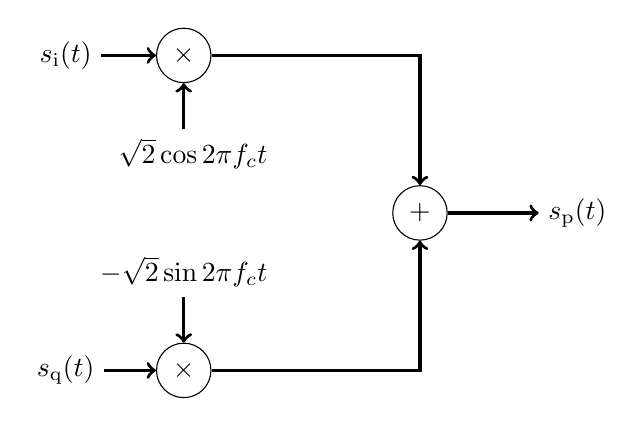
\begin{tikzpicture}[scale=1.0,transform shape]
      \node at (-0.5,2) (sc) {$s_{\text{i}}(t)$};
      \node at (-0.5,-2) (ss) {$s_{\text{q}}(t)$};
      \node[circle, draw, minimum size = 5mm] at (1,2) (prodc) {$\times$};
      \node[circle, draw, minimum size = 5mm] at (1,-2) (prods) {$\times$};
      \node[circle, draw, minimum size = 5mm] at (4,0) (adder) {$+$};
      \node at (1,0.75) (cos) {$\ \ \sqrt{2}\cos 2\pi f_ct$};
      \node at (1,-0.75) (sin) {$-\sqrt{2}\sin 2\pi f_ct$};
      \node at (6,0) (sp) {$s_{\text{p}}(t)$};
      \draw[->,very thick] (sc) -- (prodc);
      \draw[->,very thick] (ss) -- (prods);
      \draw[->,very thick] (prodc) -| (adder);
      \draw[->,very thick] (prods) -| (adder);
      \draw[->,very thick] (cos) -- (prodc);
      \draw[->,very thick] (sin) -- (prods);
      \draw[->,very thick] (adder) -- (sp);
      \end{tikzpicture}
   \caption{Up-conversion: Getting passband signal from complex envelope
   \label{fig:upconversion}}
  \end{figure}
  
    \begin{figure}
    \centering
      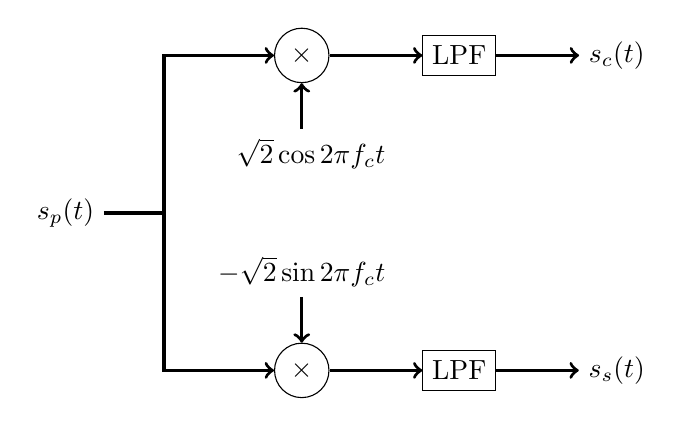
\begin{tikzpicture}[scale=1.0,transform shape]
      \node at (5,2) (sc) {$s_c(t)$};
      \node at (5,-2) (ss) {$s_s(t)$};
      \node[circle, draw, minimum size = 5mm] at (1,2) (prodc) {$\times$};
      \node[circle, draw, minimum size = 5mm] at (1,-2) (prods) {$\times$};
      \node[rectangle, draw, minimum size = 5mm] at (3,2) (LPc) {LPF};
      \node[rectangle, draw, minimum size = 5mm] at (3,-2) (LPs) {LPF};
      \node at (1,0.75) (cos) {$\ \ \sqrt{2}\cos 2\pi f_ct$};
      \node at (1,-0.75) (sin) {$-\sqrt{2}\sin 2\pi f_ct$};
      \node at (-2,0) (sp) {$s_p(t)$};
      \draw[->,very thick] (prodc) -- (LPc);
      \draw[->,very thick] (prods) -- (LPs);
      \draw[->,very thick] (LPc) -- (sc);
      \draw[->,very thick] (LPs) -- (ss);
      \draw[->,very thick] (cos) -- (prodc);
      \draw[->,very thick] (sin) -- (prods);
      \draw[->,very thick] (-0.75,0) |- (prodc);
      \draw[->,very thick] (-0.75,0) |- (prods);
      \draw[very thick] (sp) -- (-0.75,0);
      \end{tikzpicture}
      \caption{Down-conversion: Getting the complex envelope from passband
      \label{fig:downconversion}}
  \end{figure}

\section{IQ Modulator}
We have developed an IQ modulator board at Wadhwani Electronics Labs.
This IQ modulator board features Linear Technology's LTC-5598 modulator LTC-6946-1 synthesizer and PIC18F4550 microcontroller.
\begin{figure}
\centering
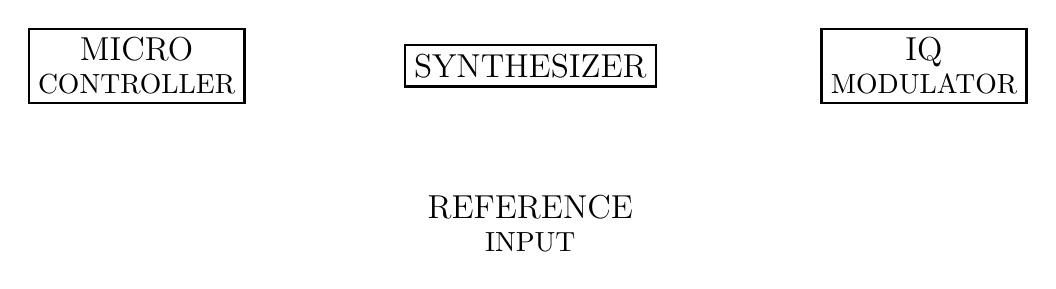
\begin{tikzpicture}[auto, thick, node distance=2cm, >=triangle 45, every text node part/.style={align=center}]
\draw
  node at (0,0)[draw, thick, rectangle]{\large MICRO \\ CONTROLLER}
  node at (5,0)[draw, thick, rectangle]{\large SYNTHESIZER}
  node at (5,-2)[]{\large REFERENCE \\ INPUT}
  node at (10,0)[draw, thick, rectangle]{\large IQ \\ MODULATOR};
\end{tikzpicture}
\end{figure}
%  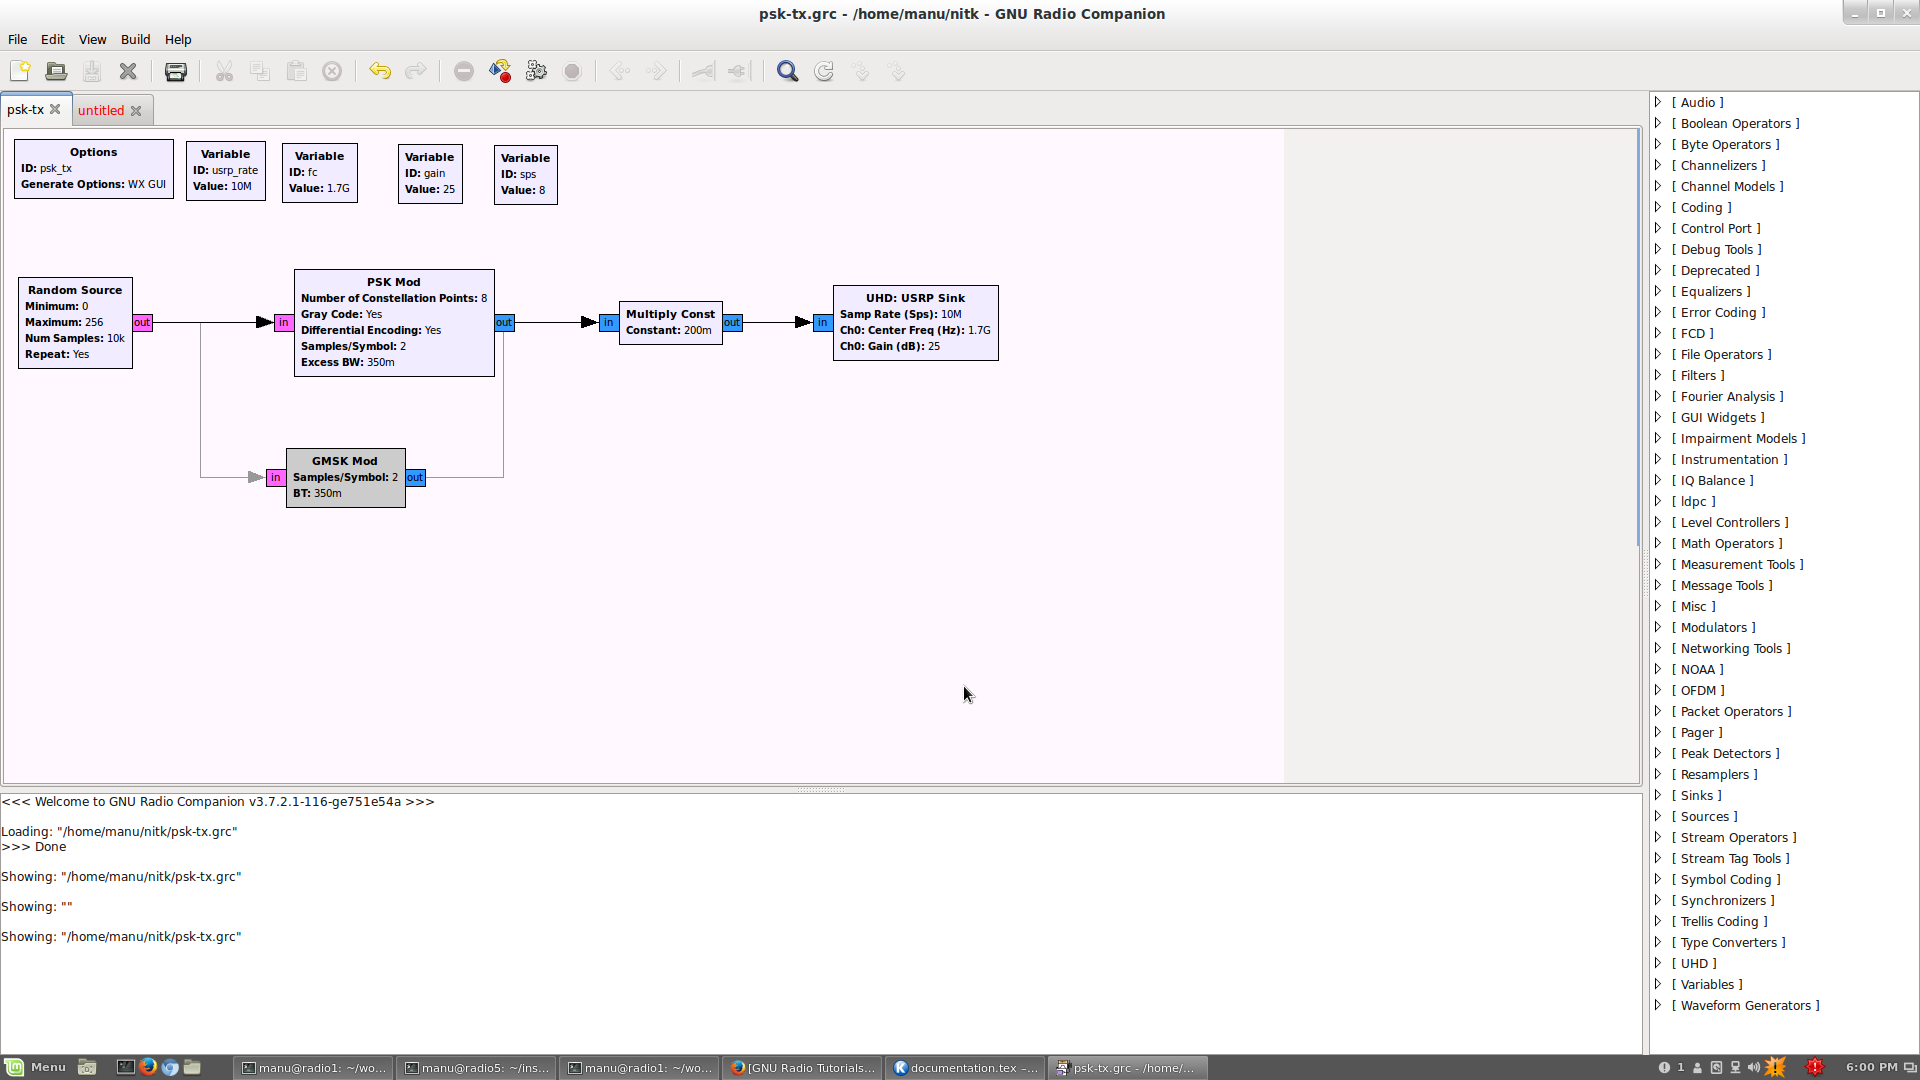
\includegraphics[scale=0.23]{figures/grc.png}
%  \caption{GNU Radio companion. The area containing the blocks in the center is the place where we assemble the flow-graphs.
%  We can drag and drop different signal processing blocks to the flow-graph from the list-box on the right.
%  The text-box on the bottom displays the output written to the terminal.\label{fig:grc}}
% \end{figure}
% \begin{figure}
% \centering
%  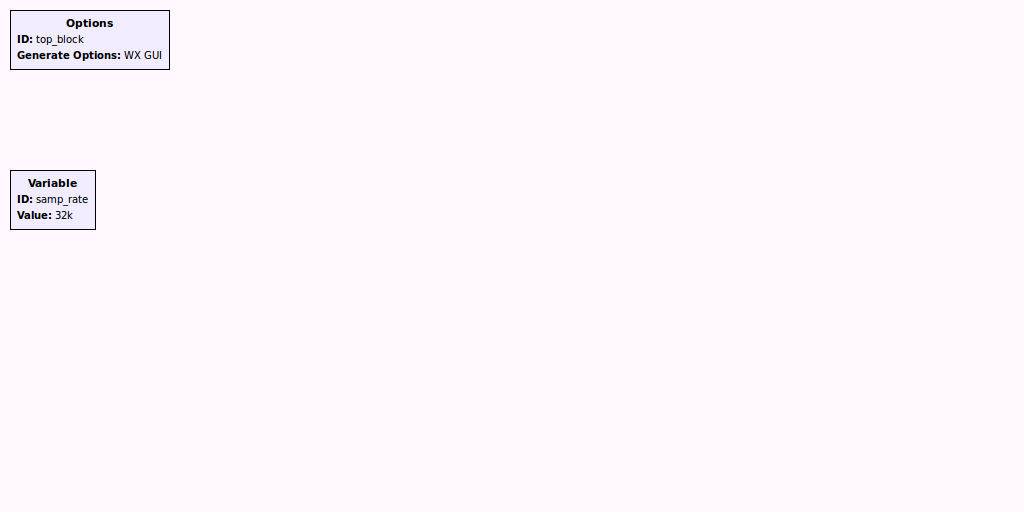
\includegraphics[scale=0.4]{figures/gnuradio-new-flowgraph.png}
%  \caption{Constructing a flow graph. On the left top we see the options block. The variable block defines a variable called samp\_rate.
%  We can change the value associated with this variable by double clicking on it and editing the property window that pops up.
%  One can use this variable in other block by putting the variable id i.e, samp\_rate.
%  \label{fig:newgraph}}
% \end{figure}


\begin{appendices}
\lstinputlisting[language=Python, caption=The python program corresponding to the flow-graph in Figure \ref{fig:audio-play1}, label=lst:audio-play1]
{flowgraphs/audioplay1.py}
\end{appendices}

% \section{IQ Modulator Board}
% The IQ modulator board features Linear Technology's LTC 5598\cite{bib:modchip}
% High Linearity Direct Quadrature
% Modulator, which works in the range from 5MHz to 1600MHz. 
% It allows direct modulation of an RF signal using differential I and Q signals.
% The I/Q baseband inputs consist of voltage-to-current converters that in turn drive double-balanced mixers.
% The outputs of these mixers are summed and applied to a buffer,
% which converts the differential mixer signals to a $50\Omega$ single-ended buffered RF output.
% 
% The carrier to the modulator is supplied from Linear Technology's LTC 6946-1\cite{bib:pllchip}, 
% an ultra-low noise and spurious integer-N synthesizer with integrated VCO. 
% This chip is a high performance, low noise phase-locked loop (PLL) with a fully integrated VCO,
% including a reference divider, phase-frequency detector (PFD) with phase-lock indicator,
% ultralow noise charge pump, integer feedback divider, and VCO output divider.
% It's frequency range is from 373MHz to 3740MHz. 
% With the combination of these chips the transmitter can communicate between 373MHz to 1600MHz.
% 
% The synthesizer can be programmed through SPI interface so as to select different frequencies of operation.
% We use microchip's PIC18F4550 as the SPI controller and also for USB interfacing.
% The modulator board is designed to work either using the USB power or from external power supply.


%%% References
\begin{thebibliography}{9}
 \bibitem{bib:gnuradio}
 \url{http://gnuradio.org}
 \bibitem{bib:modchip}
 \url{http://www.linear.com/product/LTC5598} 
 \bibitem{bib:pllchip}
 \url{http://www.linear.com/product/LTC6946} 
 
 \bibitem{bib:madhov} Upamanyu Madhov, ``Fundamentals of Digital Communication'', CUP 2008.
 
 
 \end{thebibliography}

\end{document}


